\documentclass{beamer}
\usepackage[utf8]{inputenc}
\usepackage{amsmath}
\usepackage{hyperref}
\usepackage{subcaption}
\usepackage{mathrsfs,amsmath}
\usepackage{multirow}
\usepackage{xcolor}
\usepackage{colortbl}
\setbeamercovered{highly dynamic}

\definecolor{orangebracket}{RGB}{243,115,33}
\definecolor{bluecomma}{RGB}{26,80,170}

\newcounter{saveenumi}
\newcommand{\seti}{\setcounter{saveenumi}{\value{enumi}}}
\newcommand{\conti}{\setcounter{enumi}{\value{saveenumi}}}

\resetcounteronoverlays{saveenumi}

\usetheme{CambridgeUS}
\usecolortheme{default}

%------------------------------------------------------------
%This block of code defines the information to appear in the
%Title page
\title{Natural Disasters and Financial Series}



\author[Bermudez, Juan Pablo] 
{Juan Pablo Bermudez Cespedes}

\institute[BR] 
{
  Pasante de economía\\
  Banco de la República de Colombia
}

\date[2023] % (optional)
{Octubre 2023}



%End of title page configuration block
%------------------------------------------------------------



%------------------------------------------------------------


\begin{document}

%The next statement creates the title page.
\frame{\titlepage}


%---------------------------------------------------------

\begin{frame}
\frametitle{Objetivos y Datos}
\begin{itemize}
    \item Calcular posibles efectos de desastres naturales sobre la media y la varianza de series financieras de países emergentes durante el 10 de octubre del 2004 hasta el 10 de agosto del 2022.
    \item Observar posibles diferencias en los efectos dependiendo del tipo de desastre o del país donde sucedió
    \item Las series financieras utilizadas son los Credit Default Swaps (CDS) soberanos y un índice de bolsa de cada país. 
    \item Los países a considerar son: Brazil, Chile, China, Colombia, Corea del Sur, Indonesia, Malasia, México, Perú, Sudáfrica y Turquía.
    \item Metodología usada: \textit{event study methodology.}
\end{itemize}
\end{frame}

\begin{frame}
\frametitle{Justificaciones - Media CDS}
Di Tommaso et al. (2023) \footnote{Di Tommaso, C., Foglia, M., Pacelli, V. (2023). The impact and the contagion effect of natural disasters on sovereign credit risk. An empirical investigation. International Review of Financial Analysis, 87, https://doi.org/10.1016/j.irfa.2023.102578.} expresan la función de los CDS de capturar un riesgo de liquidez inminente que los puede llevar a crisis de default posterior a un desastre natural. Ofrecen dos justificaciones para analizar el efecto de desastres naturales sobre CDS:
\begin{itemize}
     \item En el contexto actual de crisis climática evaluar los efectos de los desastres naturales en el riesgo de crédito soberano es vital.
     \item Entender el efecto será una advertencia útil para las autoridades políticas para manejar la crisis económica y social que resulta de un desastre natural.
\end{itemize}
\end{frame}

\begin{frame}
\frametitle{Justificaciones - Media CDS}
Otras justificaciones ofrecidas en la literatura son:
\begin{itemize}
    \item Zenios (2022)\footnote{Zenios, S. (2022). The risks from climate change to sovereign debt. Climatic Change 172, 30 https://doi.org/10.1007/s10584-022-03373-4. } pretende aportar al entendimiento de los efectos del cambio climático sobre la estabilidad fiscal
    \item Malluci (2022)\footnote{Mallucci, E. (2022). Natural disasters, climate change, and sovereign risk, Journal of International Economics, 139, https://doi.org/10.1016/j.jinteco.2022.103672} explica el peligro que existe en la relación entre default y acceso a mercados internacionales. Entender el efecto de los desastres naturales sobre la probabilidad de default permite al gobierno actuar para reducir la crisis económica, introduciendo instrumentos financieros para "facilitar el acceso de los gobiernos a los mercados financieros internacionales y mitigar el impacto del cambio climático".
\end{itemize}
\end{frame}

\begin{frame}
\frametitle{Justificaciones - Media Índices de bolsa}
Hay varios artículos con hipótesis del cómo afectan los desastres (naturales) a los precios de los índices:
\begin{itemize}
    \item Pagnottoni et al. (2022)\footnote{Pagnottoni P., Spelta A., Flori, A., Pammolli, F. (2022). Climate change and financial stability: Natural disaster impacts on global stock markets, Physica A: Statistical Mechanics and its Applications, 599,
https://doi.org/10.1016/j.physa.2022.127514.} citan muchos papers como el de Kaplansky y Levy (2010)\footnote{Kaplanski, G., Levy, H. (2010). Sentiment and stock prices: The case of aviation disasters, Journal of Financial Economics, 95 (2), pp. 174-201, https://doi.org/10.1016/j.jfineco.2009.10.002.} para mencionar cómo las emociones negativas por la ansiedad y el malhumor afectan el proceso de toma de decisiones de los actores del mercado, lo cual afecta la valoración de activos.
\end{itemize}
\end{frame}

\begin{frame}
\frametitle{Justificaciones - Media Índices de bolsa}
Otras justificaciones:
\begin{itemize}
    \item Giglio et al.(2021)\footnote{Giglio, S., Kelly, B., Stroebel, J. (2021). Climate finance. Annual Review of Financial Economics, 13, https://doi.org/10.1146/annurev-financial-102620-103311.} explican como la incertidumbre de los inversores frente al cambio climático y frente al rumbo de la economía justifican las fluctuaciones en el precio de los activos.
    \item De acuerdo con Pagnottoni et al. (2022), la importancia de estudiar el efecto de los desastres naturales sobre los retornos es poder generar una estrategia de cobertura en contra de los riesgos asociados a los desastres naturales.
\end{itemize}
\end{frame}

\begin{frame}
\frametitle{Justificaciones - Volatilidad}
\begin{itemize}
    \item Fakhry et al. (2018)\footnote{Fakhry, B., Aktan, B., Masood, M., Tvaronaviciene, M., Celik, S. (2018). The impact of a recent natural disaster on the Japanese financial markets: empirical evidence. Journal of Competitiveness, 10, 2,  https://doi.org/10.7441/joc.2018.02.04.} argumentan que un desastre natural genera tanta incertidumbre que vuelve a los inversionistas más aversos al riesgo, volviendo al mercado altamente volátil, con salidas de capital buscando refugio en mercados con menos incertidumbre.
    \item La aversión al riesgo se ve afectada por diversos canales, por ejemplo por la falta de información, o también por canales psicológicos\footnote{Bourdeau-Brien, M., Kryzanowski, L. (2020). Natural disasters and risk aversion. Journal of Economic Behavior \& Organization, 177, https://doi.org/10.1016/j.jebo.2020.07.007.}
\end{itemize}
\end{frame}

\begin{frame}
\frametitle{Justificaciones - Volatilidad}
\begin{itemize}
    \item Guiso et al. (2018)\footnote{Guiso, L., Sapienza, P., Zingales, L. (2018) Time varying risk aversion. Journal of Financial Economics, 128, Issue 3, 2018, https://doi.org/10.1016/j.jfineco.2018.02.007.} prueban empíricamente distintos mecanismos que afectan la aversión al riesgo, tales como cambios en la riqueza, caída en el ingreso esperado y el canal psicológico. Ellos encuentran que el miedo (inherente a choques financieros) aumentan considerablemente la aversión al riesgo.
\end{itemize}
\end{frame}

\begin{frame}{Datos}
\begin{itemize}
    \item Los CDS soberanos a 5 años para los 11 países de interés fueron extraídos de Bloomberg, mientras que los índices de bolsa fueron extraídos de varias fuentes, entre ellas investing.com, Grupo Aval, Banco de la República de Colombia, MarketWatch, Banco Central de Reserva del Perú, Yahoo Finance y Markets Insider. 
    \item Todas las series anteriores tienen frecuencia diaria, y la muestra usada comprende el periodo entre octubre 10 del 2004 a agosto 10 del 2022.
    \item Para las series de indices se revisó que no hubieran datos para días festivos usando la función \textit{is.bizday} en R para los países disponibles para la función. Para los que no estaban disponibles con la función se revisaron a mano, es decir, se creó un vector con todos los festivos durante la muestra.
\end{itemize}    
\end{frame}

\begin{frame}{Datos}
\begin{itemize}
    \item Para las series de CDS se tomó la primera diferencia para el análisis, mientras que para los índices se tomo la serie de retornos, es decir la diferencia de logaritmos 
    \item Debido a que los festivos de los distintos países no coinciden, hay varios días para los que no se tienen datos para todos los índices de bolsa. Se estableció una cantidad mínima de índices, por ejemplo 6 de 11. Si no hay datos para más de la cantidad mínima, el día en cuestión se borró de la base de datos. Por otro lado, si hay datos para al menos la cantidad mínima de índices, se realiza interpolación lineal para los índices faltantes.
\end{itemize}    
\end{frame}

\begin{frame}{Datos}
\begin{itemize}
    \item Una de las variables que usa el modelo CAPM es el retorno de mercado, para lo cual se usaron dos alternativas. En primer lugar, se realizó un promedio móvil de orden 22 siguiendo la metodología de Pagnottoni et al. (2022). En segundo lugar, para los índices de bolsa se considera también el índice MSCI Emerging Makets como retorno de mercado.
    \item Por otro lado, siguiendo a Pagnottoni et al. (2022) se agregaron como variables exógenas el PIB trimestral y el Índice de Desarrollo Financiero (FDI) anual. 
    \item Los datos del PIB real fueron extraídos de la OCDE para la mayoría de países, y para los faltantes fueron del Banco Central de Reserva de Perú, el Bureau Nacional de Estadísticas de China y el Departamento de Estadísticas de Malasia. 
\end{itemize}    
\end{frame}

\begin{frame}{Datos}
\begin{itemize}
    \item Como el ejercicio es diario, se utilizó la metodología de Chow-Lin para desagregar la serie trimestral a serie diaria, y posteriormente, se calculó la tasa de crecimiento de la serie, usando la diferencia de los logaritmos.
    \item Para el FDI (Índice de Desarrollo Financiero) se tomaron los datos del Fondo Monetario Internacional, el cual solo contaba datos hasta el 2021. Se utilizaron series de créditos de la \textit{Global Financial Development Database} para predecir el FDI para el 2022.
    \item De la misma manera que con el PIB, se estimó la serie diaria usando la desagregación temporal de Chow-Lin.
\end{itemize}    
\end{frame}

\begin{frame}{Datos}
\begin{itemize}
    \item Por último, para los desastres se utilizó la Emergency Events Database (EM-DAT) publicada por el Centro de Investigación en la epidemología de los desastres (CRED). Se descargaron todos los desastres naturales de tipo biológico, climatológico, hidrológico, geofísico y meteorológicos para la muestra de interés. 
    \item La base tiene un problema: faltan datos para el inicio y fin del desastre, y como se necesita exactitud en la fecha de inicio del desastre, se eliminaron todos los desastres que no la tuvieran, que sumaban el 6.32\% de la muestra. Es importante ver las diferencias por tipo de desastre, ya que el 68.18\% de los desastres biológicos no contaban con dia de inicio, mientras que esta proporción se reduce a 60.61\% para los climatológicos, 0.78\% para los geofísicos, 2.32\% para los hidrológicos y 5.60\% para los meteorológicos. 
\end{itemize}    
\end{frame}

\begin{frame}{Datos}
\begin{itemize}
    \item Sin embargo, se mantuvieron los desastres que no contaran con fecha de finalización, pero se les agregó de acuerdo a la duración media del tipo de desastre correspondiente.
    \item Por ejemplo: si la media de duración de todos los eventos geofísicos de la base es de 6 días, entonces si a algún desastre le falta el día final de desastre, se toma el día final como 6 días después del día de inicio.
    
\end{itemize}    
\end{frame}

\begin{frame}{Datos}
\begin{itemize}
    \item Por otro lado, teniendo en cuenta la larga duración de los desastres biológicos (158 días en promedio) y climatológicos (44 días en promedio), y siguiendo a Cavallo et al. (2021)\footnote{Cavallo, Eduardo, Becerra, Oscar and Acevedo, Laura, (2021), The Impact of Natural Disasters on Economic Growth, No 11662, IDB Publications (Working Papers), Inter-American Development Bank, https://EconPapers.repec.org/RePEc:idb:brikps:11662.}, se decidió eliminar todos los eventos biológicos y climatológicos de la base de datos,conservando solamente los geofísicos, hidrológicos y meteorológicos.

\end{itemize}    
\end{frame}

\begin{frame}{Datos}
\begin{itemize}
    \item Por último, se filtró la base de eventos para solo contar con aquellos donde el número de muertos fuese mayor a 1000 o el número de heridos fuese mayor a 1000, o el número de afectados fuese mayor a 10000, o el total de daños fuese mas a 1000 millones de dólares.
    \item El filtro anterior se hizo teniendo en cuenta el paper de Gassebner et al. (2010)\footnote{Gassebner, Martin, Keck, Alexander and Teh, Robert, (2010), Shaken, Not Stirred: The Impact of Disasters on International Trade, Review of International Economics, 18, issue 2, p. 351-368, https://EconPapers.repec.org/RePEc:bla:reviec:v:18:y:2010:i:2:p:351-368.}, el cual realiza un filtro similar, pero en vez de usar 10.000 afectados, utiliza 100.000. La diferencia en nustro acercamiento es debido a la gran reducción en desastres si se tomase 100.000 afectados como el umbral, llegando a reducir la muestra de $1503$ a apenas $322$ desastres.
\end{itemize}    
\end{frame}

\begin{frame}{Metodología - Event Study}
La metodología de estudio de eventos se trata en breves palabras de calcular el efecto de un evento en los precios de los activos (por ejemplo los retornos de un índice de bolsa). Para lo anterior se necesita realizar una estimación, generalmente previa al evento , para luego calcular retornos anormales, definidos como la diferencia del retorno observado y el retorno pronosticado por el modelo en una ventana de evento definida.\\
En la siguiente diapositiva, la Figura \ref{fig:event} presenta la estructura básica de la metodología.
\end{frame}

\begin{frame}{Metodología - Event Study}
\begin{figure}
    \centering
    \resizebox{0.8\textwidth}{!}{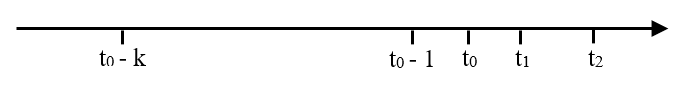
\includegraphics{Imagenes/eventstudy.png}}
    \caption{Event Study Framework}
    \label{fig:event}
\end{figure}
Donde: 
\begin{itemize}
    \item $t_0$ hace referencia al evento de interés.
    \item $[(t_0-k),(t_0-1)]$ hace referencia a la ventana de estimación.
    \item $[t_1,t_2]$ hace referencia a la ventana de evento, donde se calculan los retornos anormales. 
    \item Por el momento, para el estudio de la media realizado se han analizado las ventanas de evento donde $t_1 = t_0 + 1$, mientras que para la volatilidad se han analizado las ventanas de evento donde $t_1 = t_0$.
\end{itemize}
\end{frame}

\begin{frame}{Metodología}
\footnotesize
Siguiendo a Demirer \& Kutan (2010)\footnote{Demirer, Riza and Kutan, Ali, (2010), The behavior of crude oil spot and futures prices around OPEC and SPR announcements: An event study perspective, Energy Economics, 32, issue 6, p. 1467-1476.}, para cada desastre se corre el siguiente modelo econométrico en una ventana de estimación $[(t_0-k),(t_0-1)]$:
\begin{align}
    R_{i,t} &= \alpha +\sum_{k=1}^{p} \theta_k R_{i,t-k} +\beta_iR_t^* + \delta_iX_{i,t} + \varepsilon_{i,t} \label{rit} \\
    \eta_{i,t} &= \frac{\varepsilon_{i,t}}{\sqrt{h_{i,t}}} \sim N(0,\sigma_{i,t})  \label{epsilon}\\
    h_{i,t} &= \gamma_0+ \gamma_1 h_{i,t-1}+\gamma_2 \varepsilon_{i,t-1}^2 \label{hit}
\end{align}
Donde
\begin{itemize}
    \item $R_{i,t}$ es la serie de interés asociada al i-ésimo desastre, es decir, la serie de retornos para el caso de los índices de bolsa, y la serie en primera diferencia para los CDS.
    \item $R_t^*$ es el retorno de mercado (promedio móvil o MSCI para los índices de bolsa)
    \item $X_{i,t}$ es una matriz de variables exógenas que será definida más adelante
    \item $\varepsilon_{i,t}$ es el error no estandarizado, mientras que $\eta_{i,t}$ es el error estandarizado.
    \item $h_{i,t}$ es la varianza condicional   
\end{itemize}
\end{frame}

\begin{frame}{Metodología}
\begin{itemize}
    \item Para los estudios de la media, se va a estimar \eqref{rit}, \eqref{epsilon} y \eqref{hit} para $k = 250, 375, 500$, mientras que para la varianza será para $k=500, 750 , 1000$.
    \item Por otro lado, las ventanas de evento más grandes consideradas son $t_2=t_0+15$ para la media, y $t_2=t_0+14$ para la varianza
    \item Se procede a eliminar de la base de datos aquellos desastres que no tengan la ventana de estimación o la ventana de evento necesarias para la estimación
\end{itemize}
\end{frame}

\begin{frame}{Metodología}
\begin{itemize}
    \item Debido a que existe más de un evento catastrófico, existe la posibilidad que las ventanas de estimación de los eventos se traslapen. Algunos papers , como el de Mnasri y Nechi (2016) solucionan este problema al eliminar por completo todos los desastres que tengan dentro de su ventana de estimación cualquier otro evento.
    \item Por otro lado, muchos papers como el de Pagnottoni et al.(2022) o el de Di. Tommaso et al. (2023) no mencionan ninguna solución para el traslape de los eventos.
    \item Con la idea de no eliminar un gran número de desastres, el procedimiento que se realizó para nuestro análisis fue el siguiente:
    \begin{enumerate}
        \item Establecer una ventana de traslape, de $T_t$ días.
        \seti
    \end{enumerate}
\end{itemize}
\end{frame}

\begin{frame}{Metodología}
\begin{enumerate}
    \conti
    \item De la base de datos de eventos se escogen los eventos más significativos entre aquellos que se traslapen en una ventana de $\pm T_t$ días, definiendo la significancia como el número total de personas afectadas por el desastre.
    \item Por último, para los eventos seleccionados se corre la estimación de las ecuaciones \eqref{rit}, \eqref{epsilon}, \eqref{hit}
    \seti
\end{enumerate}
\end{frame}

\begin{frame}{Metodología}
\begin{enumerate}
    \conti
    \item Aunque no se tengan en cuenta, los eventos no seleccionados tienen efectos sobre las series que estamos estimando, por lo cual es necesario controlarlos en la regresión. La manera en que se hizo es adicionando a la ecuación \eqref{rit} una dummy que controle por este efecto. La dummy toma el valor de 1 en los días donde hubo algún otro desastre, desde que inició, hasta que terminó
    \item De este modo, las variables explicativas en \eqref{rit}, $X_{i,t}$ son la tasa de crecimiento del PIB real, la tasa de crecimiento del FDI, y la dummy que controla a los desastres que están contaminando la ventana de estimación.
\end{enumerate}
Por ejemplo, usando una ventana de estimación de k = 250 días, y una de traslape de t = 50 días, se reducen los eventos de 592 a 222.
\end{frame}

\begin{frame}{Metodología}
\begin{itemize}
    \item Posterior a la estimación de las ecuaciones \eqref{rit}, \eqref{epsilon} y \eqref{hit}, se calculan los estadísticos asociados a la metodología estudio de eventos para estudiar el efecto sobre la media y la varianza.
    \item El estudio de eventos sobre la media depende de los retornos anormales $AR_{i,t} = R_{i,t} - E[R_{i,t}]$, donde $t$ hace referencia a un día específico de la ventana de evento posterior a la ventana de estimación. $E[R_{i,t}]$ hace referencia al pronósitco del modelo para la media, con información hasta $t_0 - 1$, es decir el fin de la ventana de estimación.    
\end{itemize}
\end{frame}

\begin{frame}{Metodología}
\begin{itemize}
\item Los retornos anormales $AR_{i,t}$ pueden ser agregados a lo largo de la ventana de evento $T = t_1,...,t_2$, formando el retorno anormal acumulado $CAR_{i} = \sum_{t=t_1}^{t_2} AR_{i,t}$
    \item Por último, pueden ser promediados a nivel de evento, es decir, $CAAR=\frac{1}{N}\sum_{i=1}^{N} CAR_i$, donde N es el numero total de eventos considerados y donde $CAAR$ es el retorno anormal acumulado promedio.
\end{itemize}
\end{frame}

\begin{frame}{Metodología}
\begin{itemize}
\item Siguiendo a Savickas (2003)\footnote{Savickas, R. (2003), Event-Induced Volatility and Tests for Abnormal Performance. Journal of Financial Research, 26: 165-178. https://doi.org/10.1111/1475-6803.00052} y Demirer \& Kutan (2010)\footnote{Demirer, Riza and Kutan, Ali, (2010), The behavior of crude oil spot and futures prices around OPEC and SPR announcements: An event study perspective, Energy Economics, 32, issue 6, p. 1467-1476.} utilizamos el siguiente estadístico para evaluar la hipótesis nula $H_0: CAAR\geq0$, contra la alternativa $H_1: CAAR<0$ para los indices de bolsa o $H_0: CAAR\leq 0$, contra la alternativa $H_1: CAAR>0$ para CDS:
\begin{equation}
\text {TGarch}=\sum_{i=1}^N \frac{S_{i, T}}{N} / \sqrt{\frac{1}{N(N-1)} \cdot \sum_{i=1}^N\left(S_{i, T}-\sum_{j=1}^N S_{j, T} / N\right)^2}
\end{equation}
Donde $N$ es el número de eventos y $S_{i,T}$ está definido en la diapositiva siguiente.
\end{itemize}
\end{frame}

\begin{frame}{Metodología}

\begin{equation}
        S_{i,T} = \frac{\sum_{t=t_1}^{t_2}AR_{i,t}/(t_2-t_1+1)}{\sqrt{\sum_{t=t_1}^{t_2}\hat{h}_{i,t}/(t_2-t_1+1)}} \label{eq:sit}
    \end{equation}
Donde $t_1$ es el inicio de la ventana de evento, $t_2$ es el fin de la ventana de evento y $\hat{h}_{i,t}$ es la varianza pronosticada por el GARCH para el evento $i$ en el periodo $t$, con información hasta $t_0-1$.

\end{frame}

\begin{frame}{Metodología}
Por otro lado, tenemos el estudio sobre la volatilidad, para el cual nos basamos principalmente en el paper de Mnasri y Nechi (2016)\footnote{Mnasri, A., Nechi, S. (2016)
Impact of terrorist attacks on stock market volatility in emerging markets.
\textit{Emerging Markets Review}, 28,
\href{https://doi.org/10.1016/j.ememar.2016.08.002}{doi.org/10.1016/j.ememar.2016.08.002.}}, quienes argumentan que los residuales $\varepsilon_{i,t}$ (de la ecuación \eqref{rit}) tienen una varianza $M_t*E[h_{i,t}|\Omega_{t^*}]$ durante la ventana de evento, donde:
\begin{itemize}
    \item $E[h_{i,t}|\Omega_{t^*}]$ es la varianza condicional pronosticada por el modelo GARCH(1,1), basado en el conjunto de información $\Omega_{t^*}$, definiendo $t^* = t_0 -1$.
    \item $M_t$ es un efecto multiplicativo.
\end{itemize}

\end{frame}
\begin{frame}
\frametitle{Metodologia}
La estimación de $M_t$ es:
\begin{equation}
\widehat{M}_t=\frac{1}{N-1} \sum_{i=1}^N \frac{\left(N \times \hat{\varepsilon}_{i, t}-\sum_j^N \hat{\varepsilon}_{j, t}\right)^2}{N \times(N-2) \times E\left[h_{i, t}| \Omega_{t^*}\right]+\sum_{j=1}^N E\left[h_{j, t} \mid \Omega_{t^*}\right]},
\end{equation}

Donde $N$ es el número de eventos, $\hat{\varepsilon}_{i,t}$ son los residuales durante la ventana de evento, $E\left[h_{j, t} \mid \Omega_{t^*}\right]$ son los pronósticos de la volatilidad condicional con información hasta $t_0-1$, $t_1$ is el inicio de la ventana de evento y $t_2$ es el fin de la ventana de evento. 
\end{frame}

\begin{frame}
\frametitle{Metodologia}
Al ser un efecto multiplicativo, la hipótesis nula implica que para un día, $t > t^*$ la volatilidad no aumenta, es decir, $\hat{M_t} =1$.\\
Por lo que la hipótesis nula a lo largo de una ventana de evento $(t_1,t_2)$ va a ser: 
\begin{equation}
C A V\left(t_1, t_2\right) \equiv \left(\sum_{t=t_1}^{t_2} \widehat{M}_t\right)-\left(t_2-t_1+1\right) =0. \label{eq_cav}
\end{equation}
Donde $CAV(t_1,t_2)$ se conoce como Volatilidad Anormal Acumulada.
\end{frame}


\begin{frame}
\frametitle{Metodologia}
Por último, para calcular la significancia del $CAV(t_1,t_2)$, se realizó un bootstrap formulado por Bialkowski et al. (2008)\footnote{Bialkowski, J., Gottschalk, K., Wisniewski, T. (2008).
Stock market volatility around national elections.
\textit{Journal of Banking and Finance}, 32, \href{
https://doi.org/10.1016/j.jbankfin.2007.12.021
}{doi:10.1016/j.jbankfin.2007.12.021.}}, y perfeccionado por Mnasri y Nechi (2016).\\
Grosso modo, cada iteración del bootstrap selecciona de manera aleatoria y con reemplazo una serie de residuales para cada evento,. Los residuales escogidos son los estandarizados pero multiplicados por la volatilidad condicional pronosticada. La serie de residuales escogida para cada evento es del mismo tamaño que la ventana de evento $(t_2-t_1+1)$.\\
Posteriormente, para cada iteración se calcula el estadístico $CAV(t_1,t_2)$, definido en \eqref{eq_cav} y luego se revisa el \textit{p-value} del $CAV(t_1,t_2)$ calculado originalmente.
\end{frame}

\begin{frame}{Volatilidad Anormal Acumulada}
\framesubtitle{Resultados}
    \begin{figure}
    \begin{subfigure}{0.45\textwidth}
        \centering
        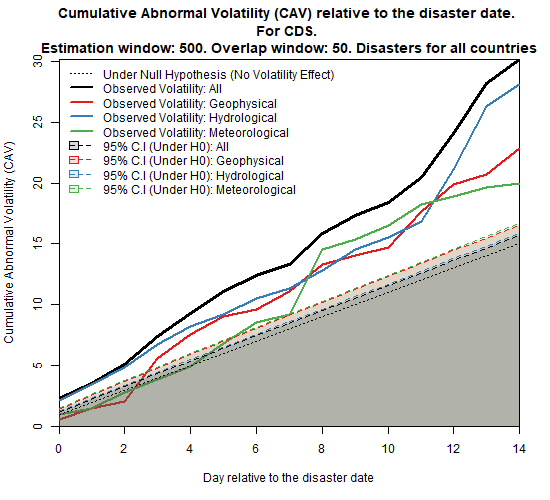
\includegraphics[width=\linewidth]{../Graficos_Paper/CAV/Ag/cds_PM_CAV_Est_500_tra_50.png}
        \caption{CAV relative to the disaster date. CDS. 500E - 50T}
        \label{figure:cavcds50050}
    \end{subfigure}
    \hfill
    \begin{subfigure}{0.45\textwidth}
        \centering
        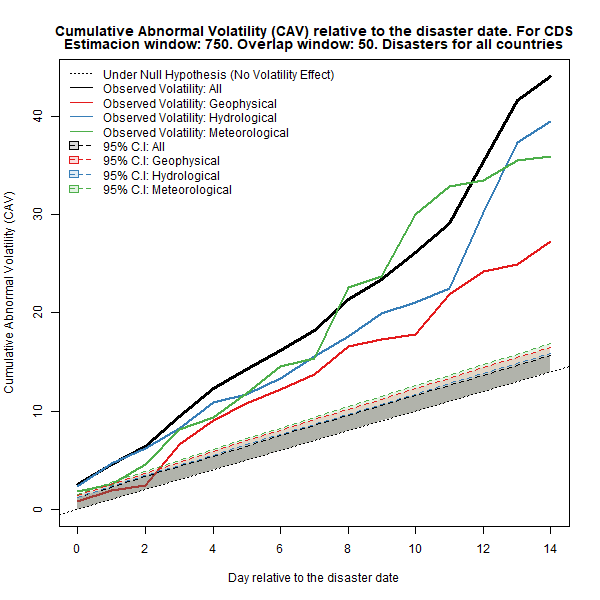
\includegraphics[width=\linewidth]{../Graficos_Paper/CAV/Ag/cds_PM_CAV_Est_750_tra_50.png}
        \caption{CAV relative to the disaster date. CDS. 750E - 50T}
        \label{figure:cavcds75050}
    \end{subfigure}
    \end{figure}
\end{frame}

\begin{frame}{Volatilidad Anormal Acumulada}
\framesubtitle{Resultados}
\begin{figure}
    \begin{subfigure}{0.5\textwidth}
        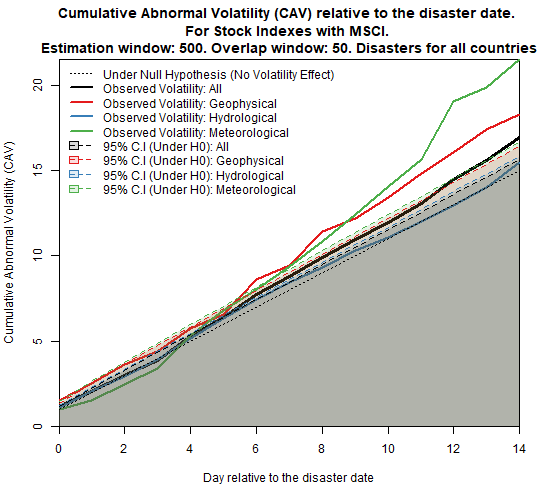
\includegraphics[width=0.9\linewidth]{../Graficos_Paper/CAV/Ag/indices_benchmark_CAV_Est_500_tra_50.png}
        \caption{CAV relative to the disaster date. Stock Indexes with MSCI, 500 E. 50 T}
        \label{figure:cavind50050}
    \end{subfigure}%
    \begin{subfigure}{0.5\textwidth}
        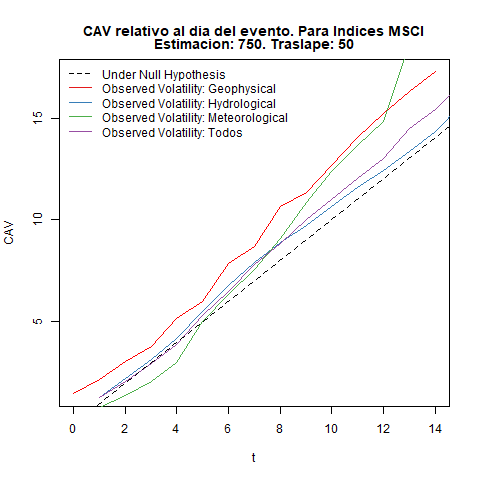
\includegraphics[width=0.9\linewidth]{../Graficos_Paper/CAV/Ag/indices_benchmark_CAV_Est_750_tra_50.png}
        \caption{CAV relative to the disaster date. Stock Indexes with MSCI, 750 E. 50 T}
        \label{figure:cavind75050}
    \end{subfigure}
\end{figure}
\end{frame}

\begin{frame}{Volatilidad Anormal Acumulada}
\framesubtitle{Resultados}
Conclusión de las gráficas de Volatilidad Anormal Acumulada (CAV) relativa al dia desastre:
\begin{itemize}
    \item Para CDS, cualquier tipo de desastre hace aumentar la volatilidad considerablemente respecto a la volatilidad pronosticada por el modelo, usando una ventana de traslape de 50 días, y una ventana de estimación de 500 o 750 días.
    \item Para los índices de bolsa usando Emerging Markets MSCI, a excepción de los desastres hidrológicos, todos los demás tipos hacen aumentar la volatilidad respecto a la volatilidad pronosticada por el modelo, usando una ventana de traslape de 50 días, y una ventana de estimación de 500 o 750 días.
\end{itemize}
\end{frame}

\begin{frame}{Resultados tests}
 A continuación se presentan los resultados de los tests econométricos mencionados anteriormente, para lo cual se tienen dos notas a tener en consideración:
 \begin{enumerate}
    \item Para todas las tablas se fija una longitud de ventana de evento de 10 días y de 15 días, es decir, para la media las ventanas de evento serán {\color{orangebracket} [1,10]} y {\color{bluecomma} [1,15]}, mientras que para la varianza serán {\color{orangebracket} [0,9]} y {\color{bluecomma} [0,14]}. Los colores serán usados en las tablas para escribir el estadístico y la significancia correspondientes a la ventana de evento del mismo color.
    \item Si ninguna de las columnas tiene ventanas significativas, igualmente se coloca el número de eventos para las ventanas de estimación y traslape correspondientes (250 E - 50 T y 500 E - 50 T para media, 500 E - 50 T y 750 E - 50 T para varianza).
 \end{enumerate}
\end{frame}

\begin{frame}{Significancia por tipo de desastre - Media}
    \begin{figure}
        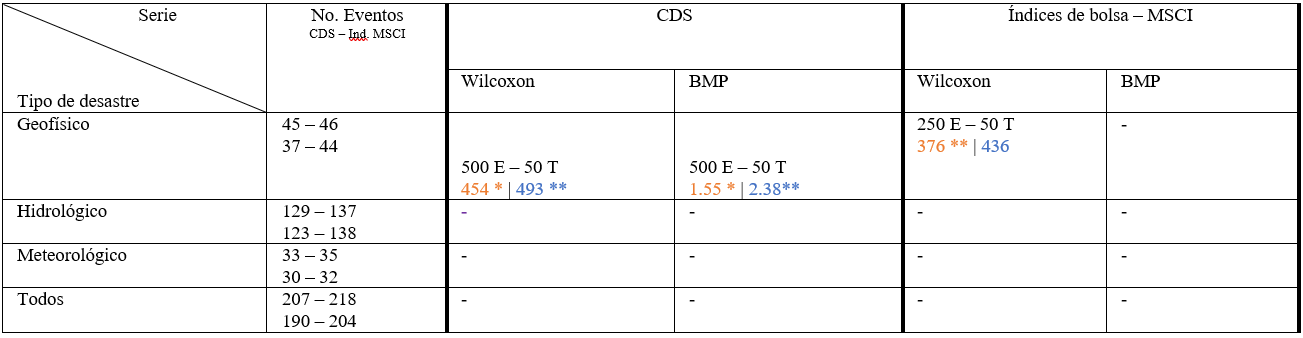
\includegraphics[width=\linewidth]{../Graficos_Paper/Tablas/Desastre_Media.png}
        \caption{Resultados tests para la media, por tipo de desastre.}
    \end{figure}
\end{frame}

\begin{frame}{Significancia por tipo de desastre - Media}
    \begin{figure}
        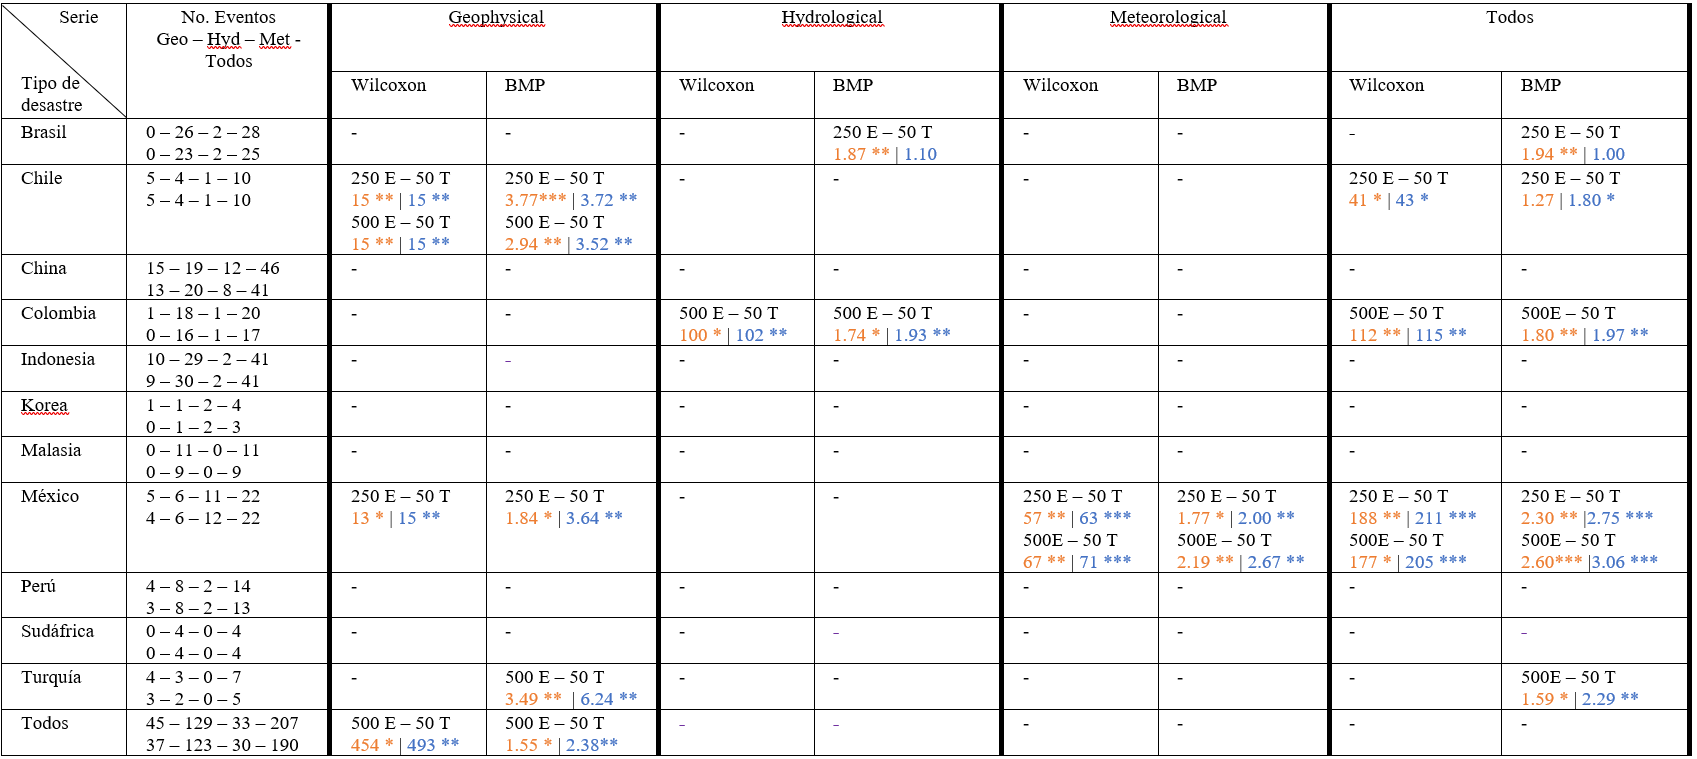
\includegraphics[width=\linewidth]{../Graficos_Paper/Tablas/Media_CDS.png}
        \caption{Resultados tests para la media para CDS}
    \end{figure}
\end{frame}

\begin{frame}{Significancia por tipo de desastre - Media}
    \begin{figure}
        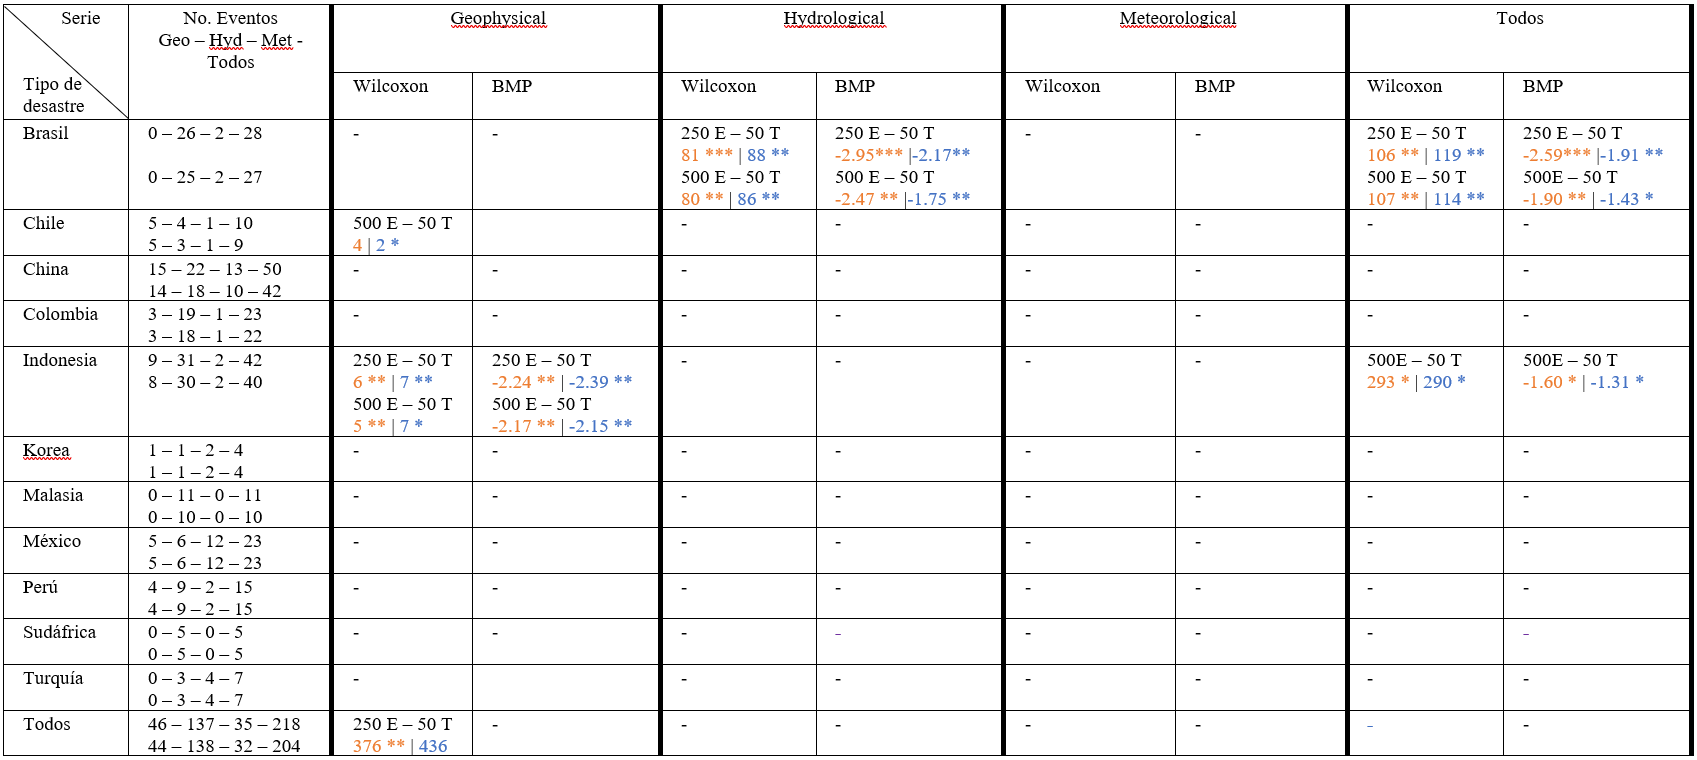
\includegraphics[width=\linewidth]{../Graficos_Paper/Tablas/Media_Stocks.png}
        \caption{Resultados tests para la media para Stocks}
    \end{figure}
\end{frame}

\begin{frame}{Significancia por tipo de desastre - Varianza}
    \begin{figure}
        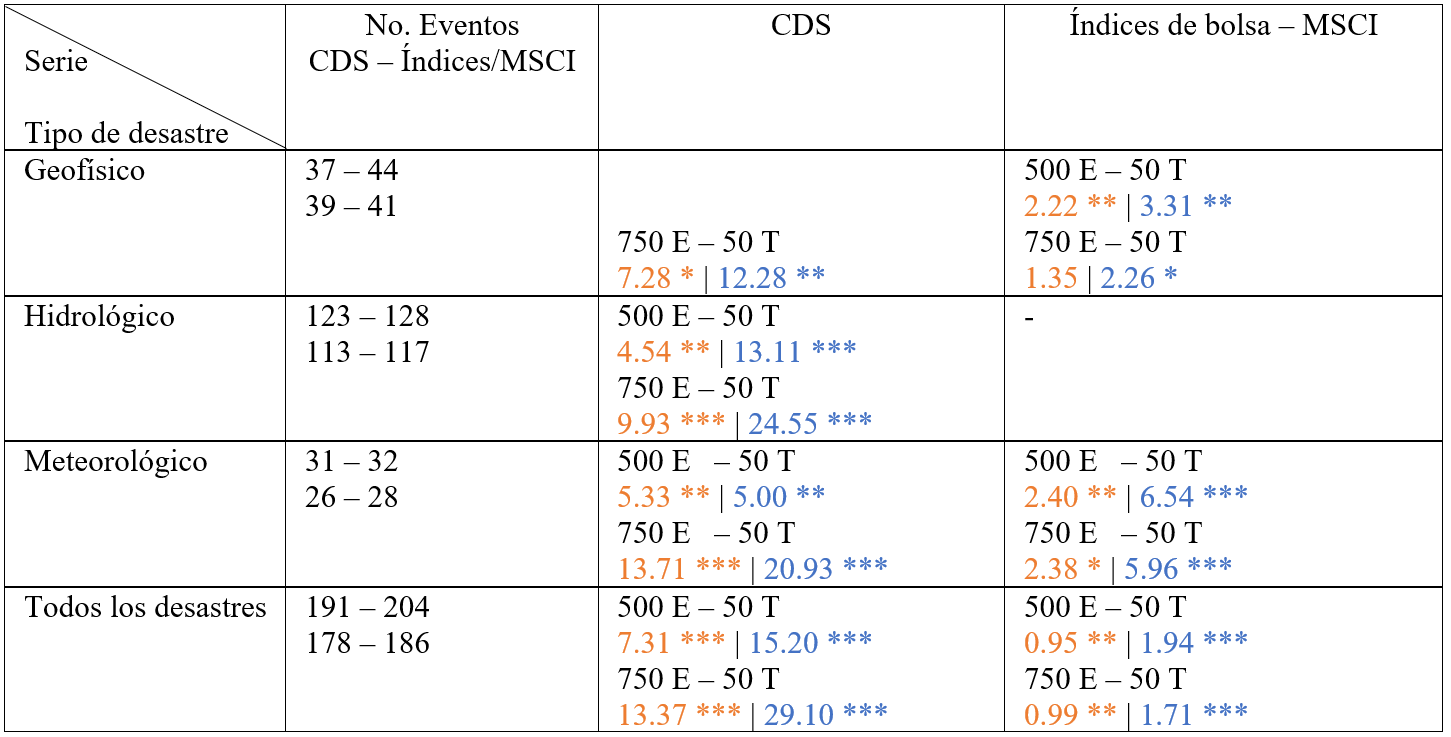
\includegraphics[width=\linewidth]{../Graficos_Paper/Tablas/Varianza.png}
        \caption{Resultados tests para la varianza, por tipo de desastre.}
    \end{figure}
\end{frame}

\begin{frame}{Significancia por tipo de desastre - Varianza}
    \begin{figure}
        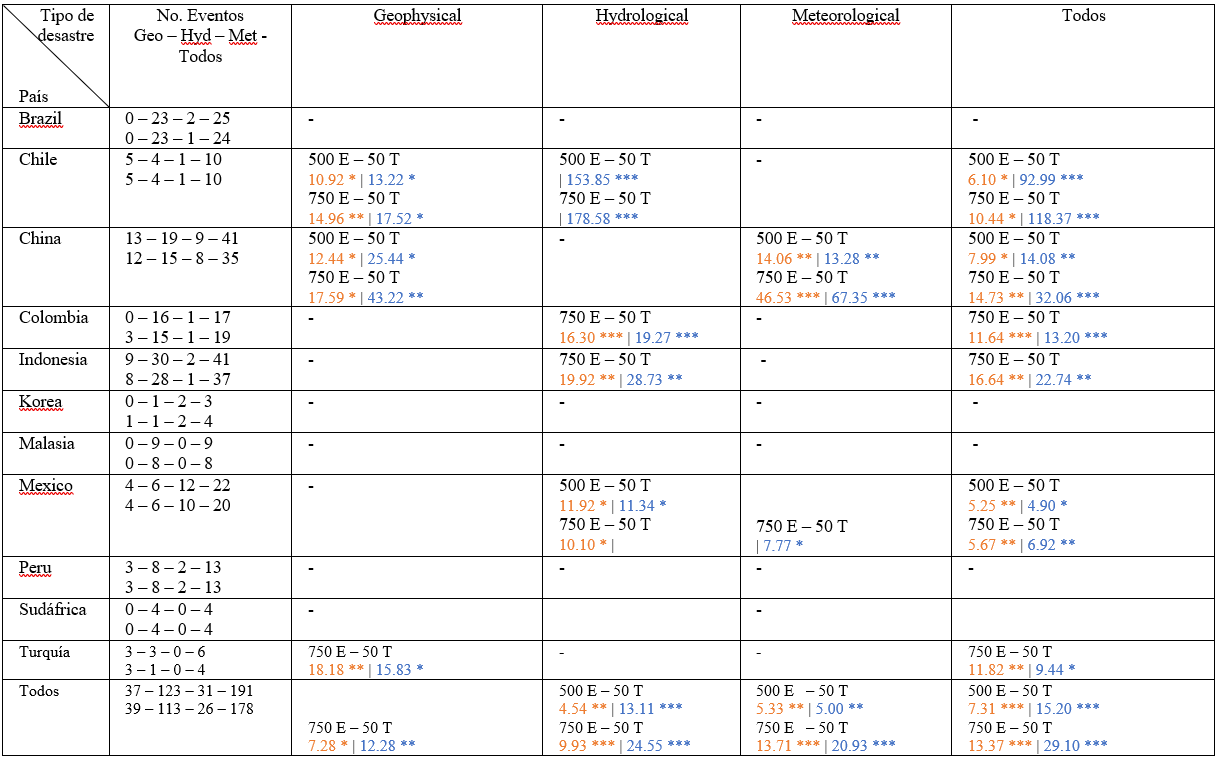
\includegraphics[width=0.9\linewidth]{../Graficos_Paper/Tablas/Varianza_CDS.png}
        \caption{Resultados tests para la varianza para CDS.}
    \end{figure}
\end{frame}

\begin{frame}{Significancia por tipo de desastre - Varianza}
    \begin{figure}
        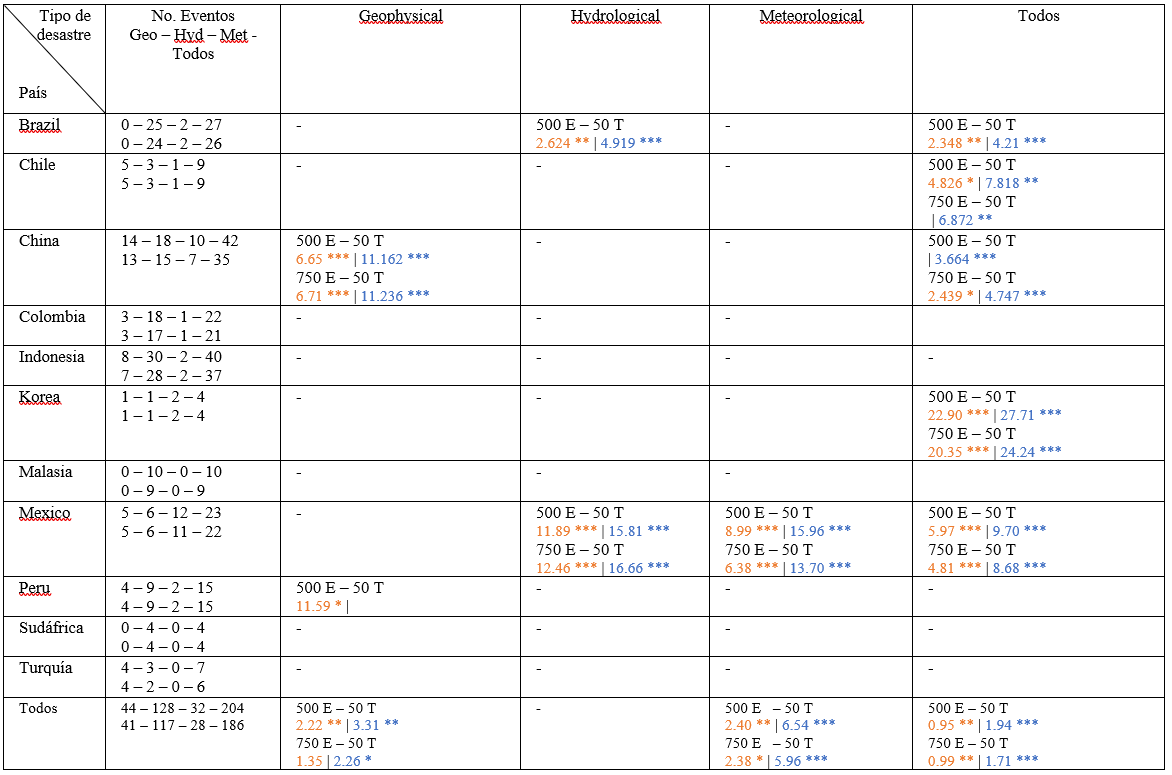
\includegraphics[width=0.9\linewidth]{../Graficos_Paper/Tablas/Varianza_Stocks.png}
        \caption{Resultados tests para la varianza para Stocks.}
    \end{figure}
\end{frame}

\end{document} 
